\begin{figure}[h!]
    \centering
    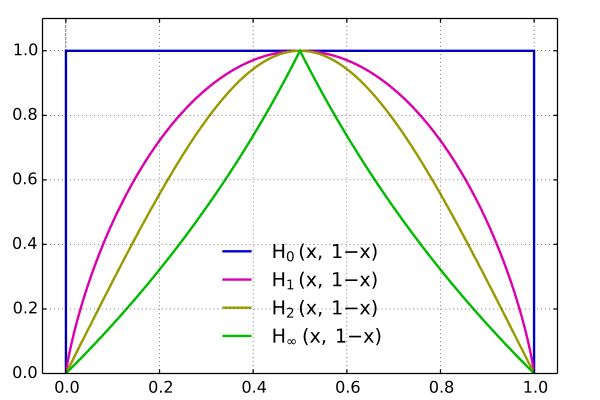
\includegraphics[width=0.6\textwidth]{figures/renyi.png}
    \caption{A comparison of Rényi entropies of different orders, plotted as they evolve on a $2$-dimensional probability vector. Here we use the result that $\lim{\alpha \rightarrow 1} H_\alpha = H$ and let the Shannon entropy be denoted by the "first-order Rényi entropy", which is here denoted as $H_1$.}
\end{figure}

\subsection{Shannon Entropy}
\label{sec:shannon}

First, we consider the most common measure of information (or "surpise"), the Shannon Entropy.

\begin{definition}
    \label{def:shannon}
    (\textbf{Shannon Entropy}) For a discrete random variable $X$, the Shannon Entropy is defined as: 
    \[H(X) = - \sum^n_{i=1}p_i \log(p_i) . \]
\end{definition}

\begin{observation}
    (\textbf{Properties of the Shannon Entropy}) The Shannon entropy has the nice property of being a (strictly) concave function, but regardless, it poses several big problems for first-order optimization methods. One big problem is that $H$ is not defined when a probability in the distribution goes to $0$ (as $\log 0$ does not exist), as $\lim_{x \rightarrow 0} x \log x = 0$ we can for convenience re-define $H$ as : 
    \begin{align*}
        H(X) := \begin{cases}
            - \sum^n_{i=1}p_i \log(p_i) & \text{if } p_1 >0 \forall i \in [n], \\
            0 & \text{otherwise. } 
        \end{cases}
    \end{align*}
    This approach "plugs" the hole in the Shannon entropy but doesn't fix all of the problems associated with. Specifically, the gradient of $H$, which is expressed as:
    \[ [\nabla H (X)]_i = - \log p_i - 1, \]
    is not Lipschitz, this is easily verifiable by observing that since $\lim_{x\rightarrow 0 a} \log(x) = -\infty$, when we pick a probability vector $\bm{p}$, s.t. for which some element $p_i \rightarrow 0$ we have that: $\| \nabla H (\bm{p})\| \rightarrow + \infty$. This makes $H$ violate an essential requirement for convergence of first-order optimization methods.
    (The gradient does have the big advantage of being separable coordinate, by coordinate, which will prove useful later.)
\end{observation}

\subsubsection{Shannon Shenanigans: Lipschitzness of the Shannon Entropy over $\Delta^{(\rho)}_n$ and contractive flow over $\mathcal{B}^n_\rho$}

The following section is sort of a detour around the Shannon Entropy properties. The fact that $H$ is non Lipschitz when some probability in the distribution goes to $0$ motivates the study of the properties of $H$ on a restricted domain, for which we guarantee that no probability $p_i$ ever goes to close to $0$, for this reason we define the $\rho$-non-vanishing simplex of dimension $n$: $\Delta^{(\rho)}_n$.

\begin{figure}[h!]
    \centering
    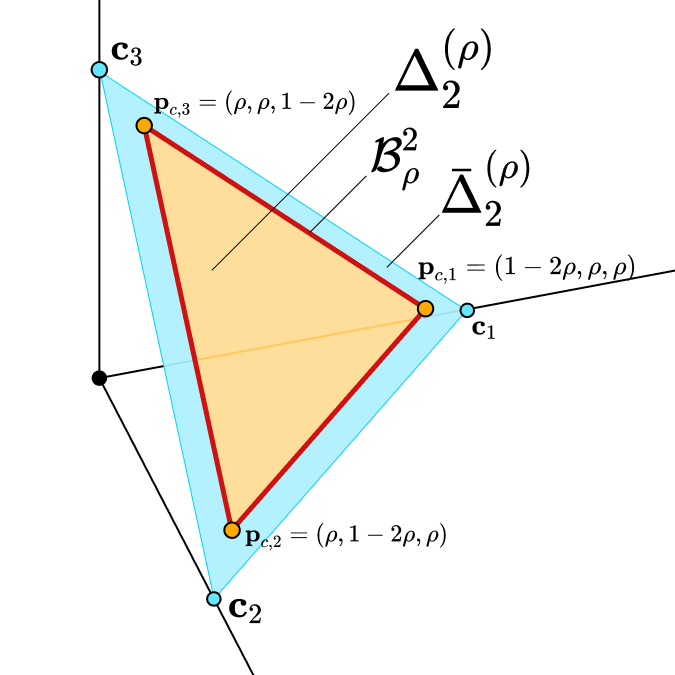
\includegraphics[width=0.6\textwidth]{figures/2-simplex.png}
    \caption{An illustration of the $2$ dimensional $\rho$ non-vanishing simplex $\Delta^{(\rho)}_n$ (the orange inner-surface, on the plot). We have that $\Delta^{(\rho)}_n \subset \Delta^2$ (the non-vanishing simplex is a subset of the simplex) and we denote on the plot the area of the simplex $\Delta^2$ that is excluded by $\Delta^{(\rho)}_n$ (i.e. $\bar{\Delta}^2_\rho = \Delta^2 \setminus \Delta^{(\rho)}_n$) in blue. The plot also labels the corners $\bm{c}_i$ of the simplex, those $\bm{p}_{c,i}$ of the non-vanishing simplex, as well as the border $\mathcal{B}^2_\rho$ of $\Delta^{(\rho)}_n$ (the red line surrounding the orange area).}
    \label{fig:2simple_nonvanishing}
\end{figure}

\begin{definition}
    \label{def:rho_non_vanishing_simplex}
    (\textbf{$\bm{\rho}$-non-vanishing Simplex}) We define "$\rho$-non-vanishing simplex" $\Delta^{(\rho)}_n$, for some $0 < \rho < 1/(n+1)$ as follows : 
    \begin{align*}
        \Delta^{(\rho)}_n := \Big\{ p \in \Delta \subset \mathbb{R}^n;~ [p]_i > \rho, ~ \forall i \in [n+1] \Big\},
    \end{align*}
    or equivalently as a convex combination over "corners" $\bm{p}_{c,i}$ of the $\rho$ non-vanishing simplex:
    \begin{align*}
        \Delta^{(\rho)}_n = \Big\{ \sum_{i\in [n+1]} \eta_i \bm{p}_{c,i},~ \sum_{i \in [n+1]} \eta_i = 1 \},
    \end{align*}
    (which will be useful when considering its border). (For a better intuition of what these spaces and objects are, refer to fig. \ref{fig:2simple_nonvanishing}) Note that the corner $\bm{p}_{c,i}$ associated with the $i$-th axes of the $n+1$ dimensional space in which $\Delta^{(\rho)}_n$ is contained has the following coordinates:
    \begin{align*}
        [\bm{p}_{c,i}]_j \begin{cases}
            1-(n+1)\cdot \rho & \text{if } j=i,\\
            \rho & \text{otherwise.}\\
        \end{cases}
    \end{align*}
    Which gives a hint of why we need to upper bound $\rho$ by $1/(n+1)$. We define the border $\mathcal{B}^n_\rho$ of $\Delta^{(\rho)}_n$ as the union of a set of $n+1$ subspaces ("edges") $\bm{E}^{(i)}$:
    \begin{align*}
        \mathcal{B}^n_\rho = \bigcup_{i\in [n+1]} \bm{E}^{(i)},
    \end{align*}
    for which each edge $\bm{E}^{(i)}_\rho$ is defined as a convex combination over all the "corners" of $\Delta^{(\rho)}_n$, excluding the $p_{c,i}$ corner:
    \begin{align*}
        \bm{E}^{(i)}_\rho = \Big\{ \sum_{j \in [n+1]\setminus i} \eta_j p_{c,j},~ \sum_{j \in [n+1]\setminus i} \eta_i = 1 \}.
    \end{align*}
    For convenience of notation we also write points on the edge $\bm{E}^{(i)}_\rho$ as a function of a parameter vector $\bm{\eta} \in \Delta^{n-1}$. In that setting we write a point on the edge as: 
    \begin{align*}
        \bm{E}^{(i)}_\rho(\bm{\eta}) = F^{(i)}_E \bm{\eta} = \sum_{j \in [n+1] \setminus i} \eta_j \bm{p}_{c,j}.
    \end{align*}
    Note that each edge is thus a convex hull on some set of corners $\bm{P}_c^{(i)} = \bm{P}_c \setminus \bm{p}_{c,i}$ of cardinality $n$ (where $\bm{P}_c$ is the set of all corners). An illustration making this more intuitive can be found in fig \ref{fig:nvsimplex_border}.
\end{definition}

\begin{figure}[h!]
    \centering
    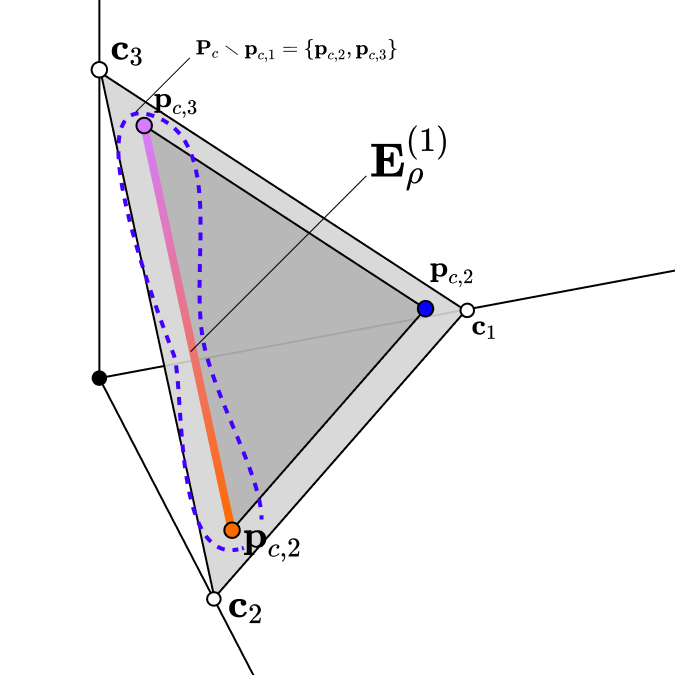
\includegraphics[width=0.6\textwidth]{figures/nvSimplexBorder.png}
    \caption{An illustration of how each edge of $\Delta^{(\rho)}_n$ is a convex-hull over a subset of $\Delta^{(\rho)}_n$'s corners.}
    \label{fig:nvsimplex_border}
\end{figure}

\begin{proposition}
    \label{prop:H_Lipschitz_over_K}
    (\textbf{$H$ is $\log(\rho^{-1})$-Lipschitz over $\Delta^{(\rho)}_n$}). 
    
\end{proposition}

\begin{proof}
    This proof is quite direct. Just observe that by definition of $\Delta^{(\rho)}_n$, which we restate below for clarity:
    \begin{align*}
        \Delta^{(\rho)}_n := \Big\{ p \in \Delta \subset \mathbb{R}^n;~ [p]_i > \rho, ~ \forall i \in [n+1] \Big\},
    \end{align*}
    we have that, if $\bm{p} \in \Delta^{(\rho)}_n$: 
    \begin{align*}
        H(\bm{p}) = - \sum^{n+1}_{i=1}p_i \log(p_i)  \leq   \sum^{n+1}_{i=1}p_i \max_{i \in [n+1]} -\log(p_i) = - \log(\rho) 
    \end{align*}
\end{proof}

Because of proposition \ref{prop:H_Lipschitz_over_K}, it would be nice to show that, under the right conditions, first-order methods ensure that steps of GD/GA/GDA stay bounded in some $\Delta^{(\rho)}_n$ for some $\rho>0$ and hence that the gradient is \textit{Lipschitz in practice} over the domain of admissible first-order steps. This is the motivation for lemma \ref{lemma:contractive_flow_of_H_over_B}.

% \subsubsection{Contractive flow of Shannon's entropy over the non-vanishing simplex border, frustration against a useless bound}
    

%     Let $H$ be Shannon's entropy and consider $\tilde{\bm{p}} \in \mathcal{B}^n_\rho$ (some element on the non-vanishing simplex border), for $0<\rho<1/(n+1)$ there exists $\beta>0$, s.t. we have:
%     \begin{align*}
%         \Big\langle \nabla H(\tilde{\bm{p}}), \frac{\partial \mathcal{B}^n_\rho(\tilde{\bm{p}})}{\partial \rho} \Big\rangle \geq \beta,
%     \end{align*}
%     where $\frac{\partial \mathcal{B}^n_\rho(\tilde{\bm{p}})}{\partial \rho}$ denotes the border-element differentiated w.r.t the non-vanishing parameter $\rho$. This statement can be read as "the flow of the gradient of $H$ flows in the same direction (or at least in some direction positively correlating with) the direction of a smaller box $\Delta^{n}_{\rho + d\rho}$". In other words our gradient flows inwards of $\Delta^{(\rho)}_n$, never outwards. See figure \ref{fig:K_border_flow} for a clearer picture.


% \begin{figure}[h!]
%     \centering
%     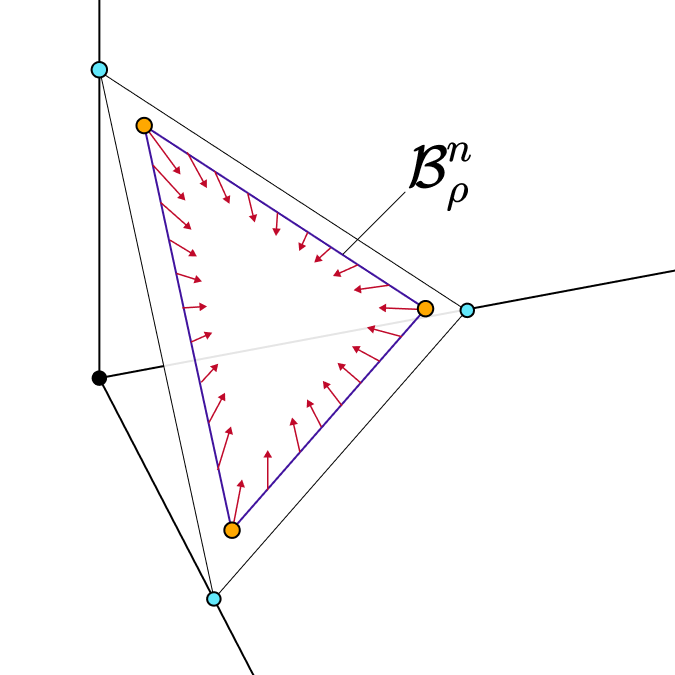
\includegraphics[width=0.6\textwidth]{figures/flowNvSimplexBorder.png}
%     \caption{Illustration in the $\Delta^{(\rho)}_n$ case of the partial derivative of the border w.r.t $\rho$ : $\frac{\partial \mathcal{B}^n_\rho(\tilde{\bm{p}})}{\partial \rho}$ (the red arrows), which is only defined on the border $\mathcal{B}^n_\rho$.}
%     \label{fig:K_border_flow}
% \end{figure}


%     We first need to explicitly compute two useful quantities: a generic element of the border $\mathcal{B}^n_\rho$, as well as the partial derivative of that element with respect to $\rho$. First, let's decompose our border $\mathcal{B}^n_\rho$ into it's individual edges, as shown in definition \ref{def:rho_non_vanishing_simplex}. Recall that we can write the full border as a union of "edges": $\mathcal{B}^n_\rho = \bigcup_{i\in [n+1]} \bm{E}^{(i)}$. Now let's observe that since the corner points are defined as:
%     \begin{align*}
%         [\bm{p}_{c,i}]_j \begin{cases}
%             1-(n+1)\cdot \rho & \text{if } j=i,\\
%             \rho & \text{otherwise.}\\
%         \end{cases}
%     \end{align*}
%     They are all permutations and since edges are all defined as convex hulls of $\bm{P}_c^{(i)} = \bm{P}_c \setminus \bm{p}_{c,i}$, we can restrict ourselves w.l.o.g to the study of a single edge element of edge $\bm{E}^{(i)}_\rho$ given by:
%     \begin{align*}
%         [\bm{E}^{(i)}_\rho(\bm{\eta})]_k = \Bigg[\sum_{j \in [n+1] \setminus i} \eta_j \bm{p}_{c,j}\Bigg]_k = \begin{cases}
%             \eta_k (1-(n+1)\rho) + \rho \sum_{j \in [n+1]\setminus k} \eta_j & \text{if } k \neq i, \\
%             \rho & \text{if } k=i.
%         \end{cases}
%     \end{align*}
%     This is quite easily differentiated w.r.t $\rho$ to give us our partial derivative $\frac{\partial \bm{E}^{(i)}_\rho(\bm{\eta})}{\partial \rho}$ for this specific edge:
%     \begin{align*}
%         \Bigg[\frac{\partial\bm{E}^{(i)}_\rho(\bm{\eta})}{\partial \rho}\Bigg]_k = 
%         \begin{cases}
%             -(n+1)\eta_k + \sum_{j \in [n+1]\setminus k} \eta_j & \text{if } k \neq i, \\
%             1 & \text{if } k=i.
%         \end{cases}
%     \end{align*}
%     For convenience we introduce here the notation $\Sigma_k =  \sum_{j \in [n+1]\setminus k} \eta_j$ for getting rid of the large sums in our derivation. Observe that since it is a convex hull, $\Sigma_k + \eta_k = 1$. Similarly we can compute the gradient of $H$ on some edge element by simply plugging the definition of our edge element into the gradient of $H$, which gives:
%     \begin{align*}
%         \Big[\nabla H(\bm{E}^{(i)}_\rho(\bm{\eta}))\Big]_k = \begin{cases}
%             \log\Big(\eta_k (1-(n+1)\rho) + \rho \Sigma_k\Big) -1 & \text{if } k \neq i, \\
%             \log\rho -1 & \text{if } k=i.
%         \end{cases}
%     \end{align*}
%     Once those quantities are well defined, it is only a matter of verifying a bound $\forall \bm{\eta} \in \Delta^{n-1}$ of the scalar product:
%     \begin{align*}
%         \Big\langle \nabla H(\bm{E}^{(i)}_\rho(\bm{\eta})), \frac{\partial\bm{E}^{(i)}_\rho(\bm{\eta})}{\partial \rho} \Big\rangle = \sum_{k \in [n+1]} \Big[\nabla H(\bm{E}^{(i)}_\rho(\bm{\eta}))\Big]_k \Big[\frac{\partial\bm{E}^{(i)}_\rho(\bm{\eta})}{\partial \rho}\Big]_k.
%     \end{align*}
%     Now observing that we have two cases, we can organize our sum in two parts, a term for the $k=i$ element and $n$ remaining terms grouped together in a sum for the other terms. We get the following expression:
%     \begin{align*}
%         \sum_{k \in [n+1]} \Big[\nabla H(\bm{E}^{(i)}_\rho(\bm{\eta}))\Big]_k \Big[\frac{\partial\bm{E}^{(i)}_\rho(\bm{\eta})}{\partial \rho}\Big]_k \\
%         = \overbrace{(-\log \rho - 1 ) }^{i=k}+ \sum_{k \in [n+1]\setminus i} 
%         \overbrace{ \Big( -1 +  \log(\eta_k (1-(n+1)\rho) + \rho \Sigma_k)\Big)}^{\Big[\nabla H(\bm{E}^{(i)}_\rho(\bm{\eta}))\Big]_k } \overbrace{\Big(-(n+1)\eta_k + \Sigma_k \Bigg)}^{\Bigg[\frac{\partial\bm{E}^{(i)}_\rho(\bm{\eta})}{\partial \rho}\Big]_k}
%     \end{align*}
%     In order to make dealing with this more manageable, we will first reorganize the sum so that the $i=k$ term distributes inside of the sum:
%     \begin{align*}
%         = \sum_{k \in [n+1]\setminus i} 
%         \Big( -1 -  \log(\eta_k (1-(n+1)\rho) + \rho \Sigma_k)\Big) \Big(-(n+1)\eta_k + \Sigma_k \Bigg) + \frac{(-\log \rho - 1 )}{n}
%     \end{align*}
%     we now have a sum over $n$ terms, we will try to find a general bound for any of these terms and our result will follow. Consider any term $\textit{(t)}_k$ of our sum: 
%     \begin{align*}
%         \textit{(t)}_k = \Big( -1 -  \log(\overbrace{\eta_k (1-(n+1)\rho) + \rho \Sigma_k}^{\textit{(i)}})\Big) \Big(\overbrace{-(n+1)\eta_k + \Sigma_k}^{\textit{(ii)}} \Big) + \frac{(-\log \rho - 1 )}{n},
%     \end{align*}
%     we can use that \textit{(i)} and \textit{(ii)} are convex hulls to get : 
%     \begin{align*}
%         \textit{(i)}\text{  :  }& 0 < \rho < \textit{(i)} < (1-(n+1)\rho) & \text{  using that $0<\rho<\frac{1}{n+1}$} \\
%         \textit{(ii)}\text{  :  }& -(n+1) < \textit{(ii)} < 1.
%     \end{align*}
%     Plugging those bounds to get an upper bound on our expression we have : 
%     \begin{align*}
%         \textit{(t)}_k &= \overbrace{(-1-\log \textit{(i)}  )}^{>0 \text{ since }\rho<1/(n+1)} \cdot \textit{(ii)}  + \frac{(-\log \rho - 1 )}{n} \\
%         & \geq (-1-\log \rho) (-n-1) + \frac{(-\log \rho - 1 )}{n} \\
%         & = (\log \rho + 1) \frac{n^2+n-1}{n}
%     \end{align*}
%     Now showing our results amounts to finding some $\rho>0$ that ensures that $\textit{(t)}_k$ is lower-bounded by $\tilde{\beta}:=\frac{\beta}{n+1}$ for $\beta>0$. We have:
%     \begin{align*}
%         && \textit{(t)}_k  \geq \tilde{\beta} \\
%         \iff && \textit{(t)}_k  \geq (\log \rho + 1) \frac{n^2+n-1}{n}  \geq \tilde{\beta}\\
%         \iff &&  \log \rho  \frac{n^2+n-1}{n}  \geq \tilde{\beta} - \frac{n^2+n-1}{n} \\
%         \iff &&  \log \rho  \geq \frac{\tilde{\beta} n}{n^2+n-1} - 1 \\
%         \iff &&  \rho  \geq \exp \Biggl( \frac{\tilde{\beta} n}{n^2+n-1} - 1 \Biggr)
%     \end{align*}

%     But this is actually quite terrible as, when $n\rightarrow + \infty$ our lower bound goes to $e^{-1}$ while the max admissible value of $\rho$ ($1/(n+1)$) really quickly goes to $0$. Which makes all of this quite useless. \textit{Maybe we can get the result by finding a tighter bound? But I probably shouldn't obsess about that...}


\subsection{Rényi Entropy}


An alternative, and more general, in a sense, definition of Entropy is that of the Rényi Entropy. It defines a large class of entropy functions with various properties.


\begin{definition}
    (\textbf{Rényi Entropy}) For a discrete random variable $X$, the Rényi Entropy of order $\alpha$ is defined as: 
    \[H_\alpha(X) = \frac{1}{1-\alpha} \log \Bigl( \sum^n_{i=1}p_i^\alpha \Bigr). \]
    Conveniently, it can also be denoted as a function of the $L_\alpha$ norm of the vector of probabilities $\bm{p}_X$ associated with the random variable $X$:
    \begin{align*}
        H_\alpha(X)= H_\alpha(\bm{p}_X)= \frac{\alpha}{1- \alpha} \log \|\bm{p}_X \|_\alpha.
    \end{align*}
\end{definition}

\begin{observation}
    (\textbf{Gradient Properties of the Rényi Entropy of order 2})
    The gradient of the Rényi entropy of order $2$ ($H_2$) is simply given by:
    \begin{align*}
        \nabla_{\bm{p}_X} H_2(\bm{p}_X) 
         = -2 \frac{ \bm{p}_X  }{\|\bm{p}_X \|_2^2}.
    \end{align*}
    And observing that, on the simplex $\Delta_n$ of dimensionality $n$ we have:
    \begin{align*}
        \|\nabla_{\bm{p}_X} H_2(\bm{p}_X)\| &= \Bigg\| -2 \frac{ \bm{p}_X  }{\|\bm{p}_X \|_2^2} \Bigg\| \\
        &= 2 \frac{ 1 }{\|  \bm{p}_X  \|_2 } \leq 2 \sqrt{n}, ~ \bm{p}_X \in \Delta_n,
    \end{align*}
    it is clear that the Rényi entropy is $2\sqrt{n}$-Lipschitz. Furthermore, when computing the eigenvalues the Hessian of $H_2$, we get:
    \begin{align*}
        \lambda_{1,2} = \frac{\pm 2}{\|\bm{p}_X \|_2^2}
    \end{align*}
    which, on the $\Delta_n$ simplex, is clearly bounded by:
    
    
    \begin{align*}
        \lambda_{1,2} = \frac{\pm 2}{\|\bm{p}_X \|_2^2} \leq \pm 2 n.
    \end{align*}
    Which shows $H_2$ to also be $2n$-smooth.
\end{observation}
% \subsection{Tsallis Entropy}